\begin{figure*}
	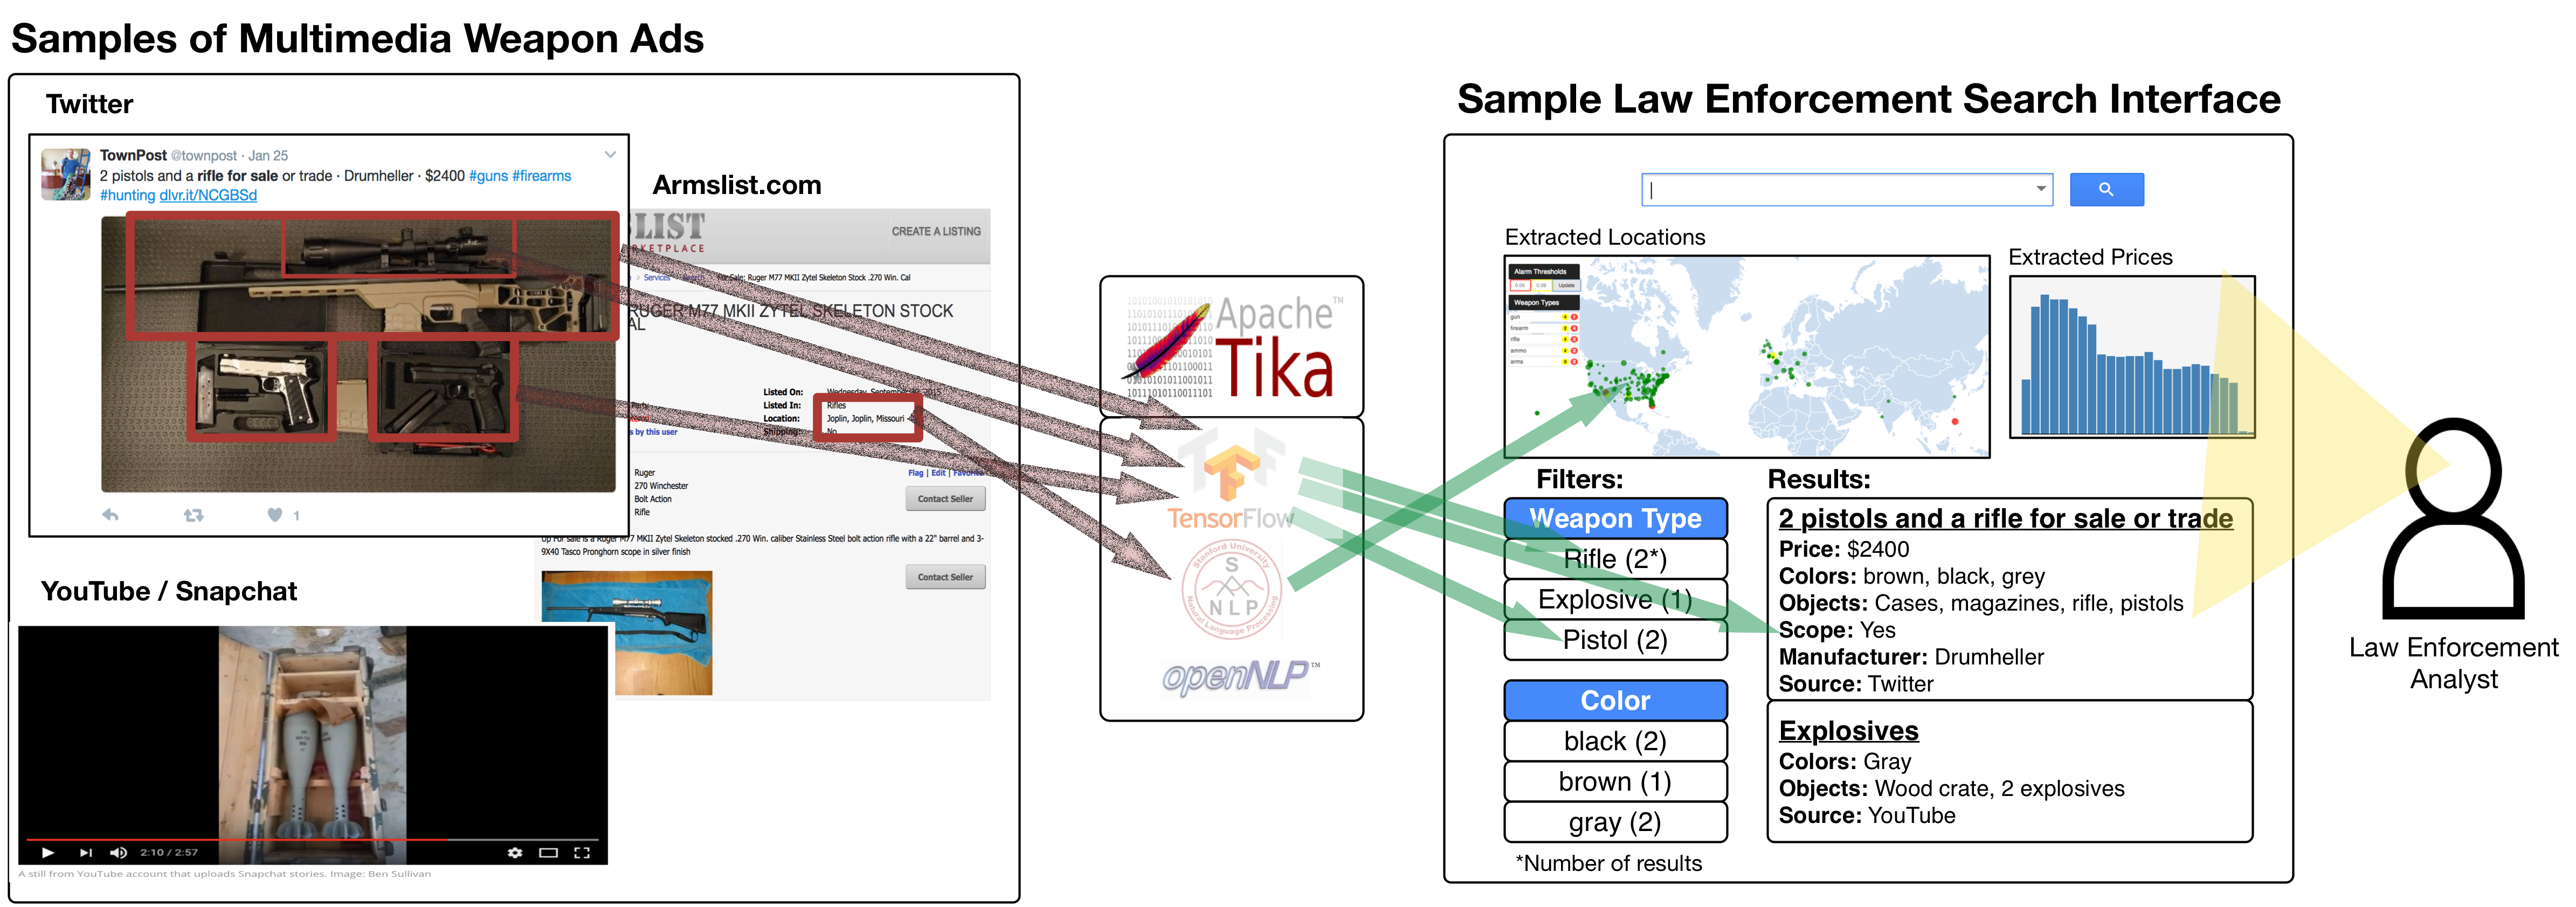
\includegraphics[width=\textwidth,height=6cm]{interface-diagram}
	\caption{This diagram demonstrates how the integration of Tika and Tensorflow facilitates interfaces in-depth search across heterogenuous content types. There are several extensions to our object recognition implementation as well, including more refined categories, optical-character recognition, and image similarity metrics.}
	\label{fig:interface-diagram}
\end{figure*}

\section{CONTENT ANALYSIS IN MEMEX PROGRAM} \label{sec:memex}
This section discusses the background and motivations of DARPA Memex program and its datasets. The current commercial web search engines provides a generalized search interface to all users~\cite{}. However, in the context of cyber security, the commercial search engines miss resources from the deep and dark web which are essential for law keeping agencies. The goal of Memex program is to develop softwares that can quickly and thoroughly organize and search subsets of information relevant to the individual interests. The first two interests were in the domains of human trafficking and illegal weapon sale.

Object recognition is a standard problem in computer vision which deals with the recognition of objects of interest in the graphical data. In the context of images it is often called as image recognition. Historically image recognition was a challenging task and its accuracy of the recognized objects were much lower than average Human performance. However, due to the recent advancements in deep neural networks and availability of larger datasets with faster computing resources, we now have systems which have nearer or better performance than average human beings\cite{karpathy-cnn-compare}.

Today's deep learning frameworks are focused towards performance gain from native code and GPU optimization for fast matrix manipulations. One of the most popular and well-documented deep-learning systems is Google's Tensorflow \cite{abadi2016tensorflow}. Tensorflow is a scalable, Python-based system and it natively supports image recognition via its {\em Inception} model \cite{abadi2016tensorflow}. Inception provides a neural network trained on the ImageNet corpus \cite{krizhevsky2012imagenet}, a dataset of 14,197,122 images and classified using the WordNet taxonomy. As such, Tensor 

 In our case, Tensorflow does not provide out of the box bindings to Java based frameworks. Apache Tika is primarily written in Java and thus integrating with Tensorflow is not straight forward like any other JVM compatible libraries. In this paper we explore various methods of integration and their pros and cons.

\subsection{Tools for Law Enforcement} \label{sec:memex-tools}
The ultimate goal of integrating diverse content scattered across the web is to provide law enforcement analysts with tools that will help them quickly identify relevant information. In the context of Memex, multimedia content is essential in helping analysts sift through millions of ads in search of illicit sales; images and videos often provide salient information not available in text. In many cases, illegal weapons dealers intentionally embed revealing details in rich content mediums because they are harder to identify. This thinking coincides with the rise of weapons trafficking on social media platforms such as Snapchat, YouTube, and Instagram, where communication is centered around images and video \cite{socialmedia}. The integration of Tensorflow and Tika provides a single, streamlined platform that unites the extraction of textual and rich content. This combined content can then be exposed through search and visualization interfaces that improve analysts' abilities to drill-down and explore comprehensive, diverse content contained in weapons ads (see Figure). Our use of Tensorflow and the Inception-V3 model serves as an example of the benefits of this integration and the types of insights and capabilities it facilitates in the future. 